% Dear Students,
% We will have the project mid-check next Monday (8th Nov). We will have a presentation and a report.
% In the presentation, each group will have 15 mins to introduce:
% 1. What is your method (methodology) to solve the problem.
% 2. What is your progress after the proposal (This will be the key part of the mid-check. 70% of the mid-check score will be given based on this.).
% 3. What is your plan for next 5 weeks.
% In the report (it should be 5-10 pages and it takes 30% of the mid-check score), you should follow the proposal style and format to
% 1. Finish the modeling (or methodology) section of the thesis (the modeling or methodology section is a temporary version. We can improve and update this part based on the experimental results).
% 2. Finish part of the implementation section.
% Thanks,
% An Zou
\documentclass[a4paper]{article}
\usepackage{amsmath,amssymb,caption,float,geometry,graphicx,indentfirst,parskip,tabularx,xcolor,listings,algorithm,algorithmic}
\usepackage{minted}
\usepackage{hyperref}
\usepackage[utf8]{inputenc}
\usepackage[english]{babel}
\usepackage[backend=bibtex]{biblatex}
\addbibresource{mid-check_report.bib}
\captionsetup[figure]{labelsep=period}
\definecolor{bg}{rgb}{0.95,0.95,0.95}
% \setlength{\parindent}{2em}
\hypersetup{
    colorlinks=true,
    linkcolor=blue,
    filecolor=blue,      
    urlcolor=blue,
    citecolor=cyan,
}
\usemintedstyle{emacs}
\begin{document}
\begin{titlepage}
    \vspace*{0.25cm}
    \noindent\rule[0.25\baselineskip]{\textwidth}{1pt}
    \begin{center}
        \huge{\textsc{UM--SJTU Joint Institute}}\vspace{0.3em}\\
        \huge{\textbf{Advanced Embedded System}}\vspace{0.3em}\\
        \Large{\textbf{(ECE4730J)}}
        \noindent\rule[0.25\baselineskip]{\textwidth}{1pt}
    \end{center}
    \begin{center}
        \vspace{5cm}
        \LARGE{\textsc{Mid-Check Report}}\vspace{0.5em}\\
        \Large{\textbf{ELMA: Encrypted Offloading for Embedded NLP Applications}}\vspace{1em}\\
        \Large{\textbf{Group 3}}\\
    \end{center}
    \vfill
    \large
    \begin{tabular}{ll}
        Name: Yihua Liu \hspace*{2em}&ID: 518021910998\hspace*{2em}\\
        Name: Yiming Ju \hspace*{2em}&ID: 518370910059\hspace*{2em}\\
        Name: Shuocheng Chen \hspace*{2em}&ID: 517021911139\hspace*{2em}\\
        \\
        Date: \today
    \end{tabular}
\end{titlepage}
\tableofcontents
\newpage
\section{Overview}

The project can be divided into three parts, including the full model on the remote server, the lite model on local embedded system and the link between the server and the embedded device. 

\section{Methodology}
\begin{figure}[H]
    \centering
    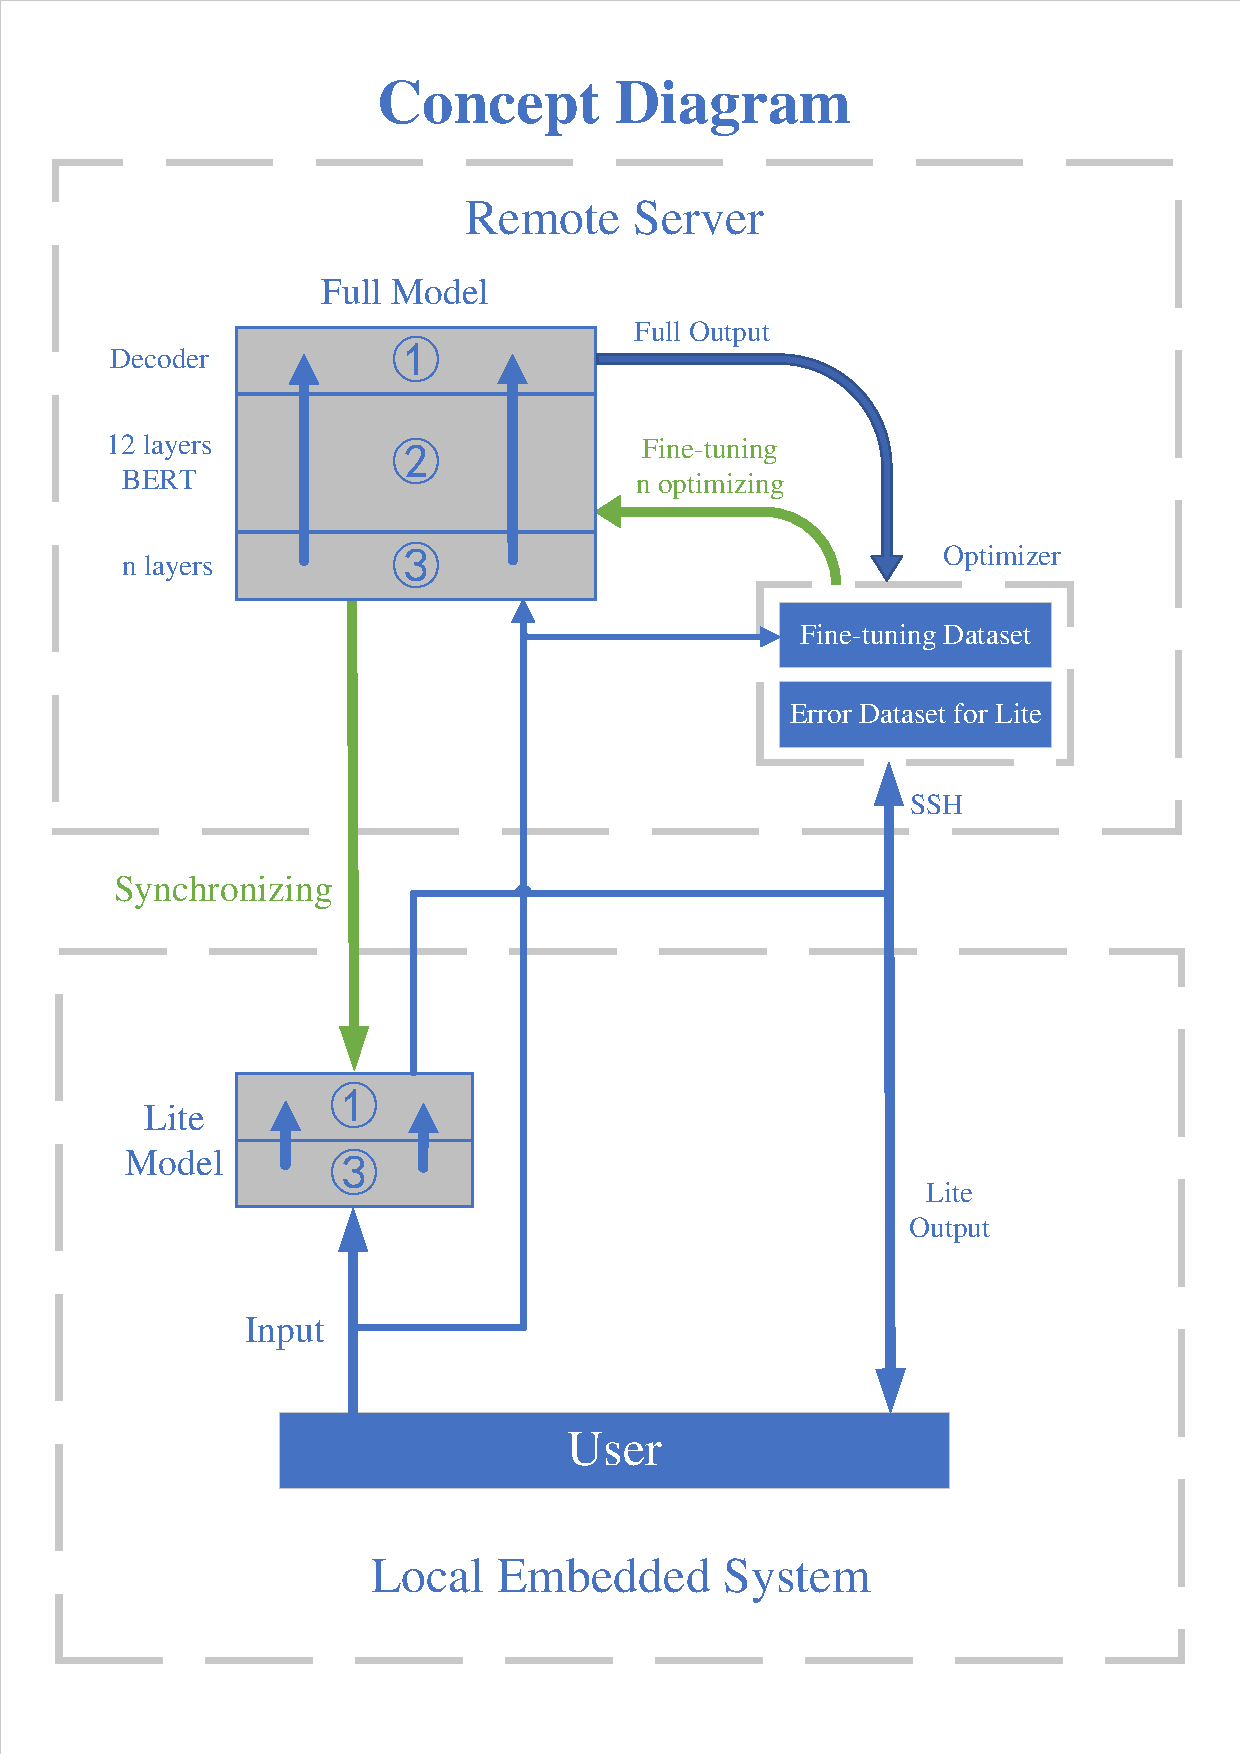
\includegraphics[width=0.5\textwidth]{Concept_Design.pdf}
    \caption{The diagram of the concept design.}
\end{figure}
\subsection{Full ALBERT Model}
ALBERT\cite{lan2020albert} is a model based on BERT with better performance. A pre-trained model of ALBERT\cite{lan2020albert} will be used in our project and it will be fine-tuned on the dataset SQuAD\cite{squad2.0}. It is expected to be 12 layers in the model.

\subsection{Lite EdgeBERT Model}
Since the size of 12 layers is still too large for embedded systems, a lite model with less layers will be preferred. Thus an abridged ALBERT model with about 5 layers will be used in our embedded system. Its advantages are to prevent over-fitting and reduce computation. Between each two layers, there will be a classification layer so as to check whether the output is accurate enough to satisfy the need. In this way, complex sentences will be with larger model while simple sentences will be with smaller one. Depending on the structural and contextual complexity, a given input can exit earlier or later. \\
To evaluate the standard quantitatively, a concept named entropy is defined below \cite{tambe2021edgebert}
\begin{equation}
H(x)=-\sum p(x)\log{p(x)}=\ln{(\sum^n_{k=1}e^{x_k})}-\frac{\sum^n_{k=1}x_k e^{x_k}}{\sum^n_{k=1}x_k}
\end{equation}
Then \textbf{Algorithm 1} indicates how to realize early exit in lite model.
\begin{algorithm}
\caption{Early Exit} 
\label{alg1}
\begin{algorithmic}
\FOR{layer i from 1 to n do}
\IF{$H(z_i)<E_T$} 
\RETURN{$z_i$}
\ENDIF 
\ENDFOR
\IF{the question is solved} 
\RETURN{$z_n$}
\ELSE
\RETURN{unsolvable question to the remote server}
\ENDIF 
\end{algorithmic}
\end{algorithm}\\
where $z_i$ is the output of each transformer layer and $E_T$ is the threshold to exit. Once the value of entropy is smaller than the threshold, the model will exit early and output the result.

\subsection{Link between two models}
The link between the full model and the lite model is bidirectional. At the end of the lite model, the output will be checked whether the question is answerable locally. Otherwise it will be uploaded to the remote server as the data in error data set for lite model, which is to make the model more corresponding to the local needs. In turn, the local lite model will be optimized through synchronizing the model, which is trained by the unsolvable questions from lite model.


\section{Implementation and Validation}
Our system is similar to an edge computing system, while only one edge device is applied as an embedded platform. validation environment contains two parts: the embedded platform and the cloud platform.
\subsection{Validation Environment of Embedded Platform}
NVIDIA Jetson TX2 serves as the embedded platform. Jetson TX2 is an embedded computing device for artificial intelligence.
\subsubsection{Hardware Specifications}
The embedded platform uses the following hardware specifications:
\begin{enumerate}
    \item GPU: 256-core NVIDIA Pascal GPU architecture with 256 NVIDIA CUDA cores
    \item CPU: Dual-core 64-bit NVIDIA Denver 2 CPU and quad-core ARM Cortex-A57 MPCore
    \item Memory: 8\,GiB 128-bit LPDDR4
    \item Storage: 32\,GiB eMMC 5.1 and 512\,GiB SATA 3.0
\end{enumerate}
\subsubsection{Development Environment}
NVIDIA provides a software development kit for Jetson platforms called JetPack SDK. The embedded platform is based on JetPack 4.6, which includes the following components:
\begin{enumerate}
    \item Ubuntu 18.04.6 LTS (bionic) with Linux kernel 4.9.253-tegra
    \item CUDA Toolkit 10.2 for L4T
    \item \texttt{cuDNN} 8.2.1
    \item \texttt{TensorRT} 8.0.1-1+cuda10.2 (8.0.1.6)
\end{enumerate}
\subsubsection{Package Dependencies}
Since TensorFlow does not provide builds for AArch64 (ARMv8) architecture with GPU support, TensorFlow is manually compiled, built, and installed from GitHub source of branch \texttt{v2.7}.
\begin{enumerate}
    \item \texttt{gcc (Ubuntu/Linaro 7.5.0-3ubuntu1~18.04) 7.5.0}
    \item Python 3.6.9
    \item Anaconda 4.10.1 (Python 3.8.8, GCC 10.2.0)
    \item Bazel 3.7.2 (from \texttt{npm} package \texttt{@bazel/bazelisk} 1.10.1)
\end{enumerate}
\subsection{Validation Environment of Cloud Platform}
The cloud platform is based on VMware vSphere Bitfusion servers. Virtual desktops (clients) are provided individually by JI IT Office and the access to GPU resources is guaranteed by Bitfusion utilities in the Virtual Desktops.
\subsubsection{Hardware Specifications}
The embedded platform uses the following hardware specifications:
\begin{enumerate}
    \item GPU: 4*2 Tesla V100 32GiB GPU with NVIDIA Volta architecture and 640 NVIDIA tensor cores on Bitfusion Cloud Server
    \item CPU: Quad-core Intel Xeon Gold 6226 @ 2.70GHz
    \item Memory: 8GiB 32-bit VMware Virtual Memory
    \item Storage: 200GiB VMware Virtual Disk
\end{enumerate}
\subsubsection{Development Environment}
VMware vSphere Bitfusion client provides the following components:
\begin{enumerate}
    \item Ubuntu 20.04.3 LTS (focal) with Linux kernel 5.11.0-38-generic
\end{enumerate}
To run dated packages, e.g, the original release of Albert, two sets of environments are installed to satisfy different requirements.
\begin{enumerate}
    \item Original Release of Google Albert
    \begin{enumerate}
        \item CUDA Toolkit 10.0
        \item CuDNN 7.4.0
    \end{enumerate}
    \item Transformer Repository from Hugging Faces
    \begin{enumerate}
        \item CUDA Toolkit 11.2
        \item CuDNN 8.1.0
    \end{enumerate}
\end{enumerate}


\subsubsection{Package Dependencies}
Common NLP requirements, e.g., numpy and sentencepiece, are omitted.
\begin{enumerate}
    \item Original Release of Google Albert
        \begin{enumerate} 
            \item Python 3.6.15
            \item Tensorflowgpu 1.15.2
            \item CuPy 9.5.0 for CUDA 10.0
        \end{enumerate}
    \item Transformer Repository from Hugging Faces
        \begin{enumerate} 
            \item Python 3.8.10
            \item Tensorflow 2.7.0
            \item CuPy 9.5.0 for CUDA 11.2
        \end{enumerate}
\end{enumerate}

\section{Problems and Solutions}
\subsection{Embedded Platform}
\subsubsection{Compability and Dependency}
\begin{enumerate}
    \item Problem: Bazel does not provide binaries for AArch64/ARMv8.\\
    Solution:\\
    For TensorFlow 1.15.2 requires Bazel 0.26.1, so we have to manually compile and build Bazel by Scratch
    \begin{minted}[frame=single,bgcolor=bg,breaklines]{bash}
sudo apt-get install build-essential openjdk-11-jdk python zip unzip
cd bazel-0.26.1-dist
find -name '*.sh' -exec chmod a+x '{}' \;
sudo -E env EXTRA_BAZEL_ARGS="--host_javabase=@local_jdk//:jdk" bash ./compile.sh
    \end{minted}
    We have to manually change the permission settings of all the shell scripts because they are not executable by default after extracting from the distribution zip file.\\
    For TensorFlow 2.7, we can directly install Bazel 3.7.2 from bazelisk 1.10.1
    \begin{minted}[frame=single,bgcolor=bg,breaklines]{bash}
npm install -g @bazel/bazelisk
    \end{minted}
    \item Problem: TensorFlow does not provide binaries for AArch64/ARMv8.\\
    Solution: manually compile and build TensorFlow.\\
    Take TensorFlow 2.7 as example,
    \begin{minted}[frame=single,bgcolor=bg,breaklines]{bash}
git clone https://github.com/tensorflow/tensorflow.git
cd tensorflow
git checkout r2.7
sudo .configure
sudo -E bazel --output_user_root=/ssddata/bazel build --config=dbg --config=cuda //tensorflow/tools/pip_package:build_pip_package
    \end{minted}
    \item Problem: TensorFlow 1.15.2 pre-built configuration configuration asks for Open MPI, ComputeCPP, and \texttt{clang} support.\\
    Solution:
        \begin{minted}[frame=single,bgcolor=bg,breaklines]{bash}
tar -xf ComputeCpp-CE-2.7.0-aarch64-linux-gnu.tar
cd ComputeCpp-CE-2.7.0-aarch64-linux-gnu
sudo mv ComputeCpp-CE-2.7.0-aarch64-linux-gnu /usr/local
sudo mv /usr/local/ComputeCpp-CE-2.7.0-aarch64-linux-gnu /usr/local/computecpp
sudo sed -i '\$a deb http://apt.llvm.org/bionic/ llvm-toolchain-bionic main\ndeb-src http://apt.llvm.org/bionic/ llvm-toolchain-bionic main' /etc/apt/sources.list
sudo apt-key adv --keyserver keyserver.ubuntu.com --recv-keys 15CF4D18AF4F7421
sudo apt update
sudo apt install clang-format clang-tidy clang-tools clang clangd libc++-dev libc++1 libc++abi-dev libc++abi1 libclang-dev libclang1 liblldb-dev libllvm-ocaml-dev libomp-dev libomp5 lld lldb llvm-dev llvm-runtime llvm python-clang
gunzip -c openmpi-4.1.1.tar.gz | tar xf -
cd openmpi-4.1.1
sudo ./configure --prefix=/usr/local
sudo make all install
        \end{minted}
    \item Problem: TensorFlow 1.15.2 pre-build configuration \_\_main\_\_.UserInputError: SYCL / CUDA / ROCm are mututally exclusive. At most 1 GPU platform can be configured.\\
    Solution: Do not choose ROCm, OpenCL SYCL, and CUDA simultaneously. Only CUDA is needed.
    \item Problem: TensorFlow pre-built configuration requires specifying CUDA compute capabilities.\\
    Solution: According to \href{https://developer.nvidia.com/cuda-gpus}{CUDA GPUs | NVIDIA Developer}, the CUDA compute capability of Jetson TX2 is 6.2.
    \item Problem: TensorFlow pre-built configuration ERROR: Config value download\_clang\_use\_lld is not defined in any .rc file.\\
    Solution: use \texttt{gcc} instead of \texttt{clang}. All of the tested build configuration for Linux provided by TensorFlow use \texttt{gcc}.
    \item Problem: TensorFlow 1.15.2 building ValueError: dictionary update sequence element \#9 has length 1; 2 is required.\\
    Solution: At Line 355 of third\_part/gpus/find\_cuda\_config.py, specify \texttt{cudnn\_version} to be 8.
    \item Problem: TensorFlow 1.15.2 building Illegal ambiguous match on configurable attribute "deps" in //tensorflow/tools/pip\_package:included\_headers\_gather.\\
    Solution: Again use \texttt{gcc} instead of \texttt{clang}.
    \item Problem: TensorFlow 1.15.2 building error: overriding 'virtual void ... noexcept'.\\
    Solution:\\
    Change the prototype of function \texttt{log} at Line 26 of tensorflow/compiler/tf2tensorrt/utils/trt\_logger.h from
    \begin{minted}[frame=single,bgcolor=bg,breaklines]{cpp}
void Logger::log(Severity severity, const char* msg)
    \end{minted}
    to
    \begin{minted}[frame=single,bgcolor=bg,breaklines]{cpp}
void log(Severity severity, nvinfer1::AsciiChar const* msg) noexcept
    \end{minted}
    \item Problem:\\
    TensorFlow 1.15.2 building error: declaration of 'void* createInferRuntime\_INTERNAL(void*, int)' has a different exception specifier.\\
    Solution: Change the prototype of function \texttt{getLogger} at Line 19 and Line 26 of tensorflow/compiler/tf2tensorrt/stub/NvInfer\_5\_0.inc from
    \begin{minted}[frame=single,bgcolor=bg,breaklines]{cpp}
nvinfer1::ILogger* getLogger()
    \end{minted}
    to
    \begin{minted}[frame=single,bgcolor=bg,breaklines]{cpp}
nvinfer1::ILogger* getLogger() noexcept
    \end{minted}
    and change the prototype of function \texttt{getPluginRegistry} at Line 33 and Line 40 of tensorflow/compiler/tf2tensorrt/stub/NvInfer\_5\_0.inc from
    \begin{minted}[frame=single,bgcolor=bg,breaklines]{cpp}
nvinfer1::IPluginRegistry* getPluginRegistry()
    \end{minted}
    to
    \begin{minted}[frame=single,bgcolor=bg,breaklines]{cpp}
nvinfer1::IPluginRegistry* getPluginRegistry() noexcept
    \end{minted}
    \item Problem: TensorFlow 1.15.2 building cudnnGetRNNDescriptor error.\\
    Solution: Change \texttt{cudnnGetRNNDescriptor} into \texttt{cudnnGetRNNDescriptor\_v6} or change
    \begin{minted}[frame=single,bgcolor=bg,breaklines]{cpp}
RETURN_IF_CUDNN_ERROR(cudnnGetRNNDescriptor(
    /*handle=*/cudnn.handle(), /*rnnDesc=*/rnn_desc,
    /*hiddenSize=*/&hidden_size_v,
    /*numLayers=*/&num_layers_v,
    /*dropoutDesc=*/&dropout_desc,
    /*inputMode=*/&input_mode,
    /*direction=*/&direction,
    /*mode=*/&mode,
    /*algo=*/&algo,
    /*dataType=*/&data_type));
    \end{minted}
    into
    \begin{minted}[frame=single,bgcolor=bg,breaklines]{cpp}
cudnnDataType_t data_type, mathPrec;
cudnnRNNMode_t cellMode;
cudnnRNNBiasMode_t biasMode;
cudnnMathType_t mathType;
int32_t inputSize, projSize;
uint32_t auxFlags;
RETURN_IF_CUDNN_ERROR(cudnnGetRNNDescriptor_v8(
    rnn_desc,
    &algo,
    &cellMode,
    &biasMode,
    &direction,
    &input_mode,
    &data_type,
    &mathPrec,
    &mathType,
    &inputSize,
    &hidden_size_v,
    &projSize,
    &num_layers_v,
    &dropout_desc,
    &auxFlags));
    \end{minted}
    \item Problem: TensorFlow 1.15.2 building error: 'cudnnConvolutionFwdPreference\_t' was not declared in this scope.\\
    Solution: Migrate to TensorFlow 2.7 because this incompatibility is un-resolvable. According to Table 7. API functions and data types that were removed of Nvidia cuDNN Documentation, \texttt{cudnnConvolutionFwdPreference\_t} is removed since cuDNN version 8.
    \item Problem: the recommended GCC version is 7.3.1 but this version is not installed.\\
    Solution:
    \begin{minted}[frame=single,bgcolor=bg,breaklines]{bash}
sudo mkdir /etc/apt/sources.list.d
sudo add-apt-repository ppa:jonathonf/gcc
sudo apt-get update
sudo apt install gcc-7
    \end{minted}
    If the directory /etc/apt/sources.list.d does not exist, it will prompt "no such file or directory" error when adding APT repository.
    \item Problem: TensorFlow 2.7 building crosstool\_wrapper\_driver\_is\_not\_gcc failed.\\
    Solution: remove option \texttt{--config=v1} of \texttt{bazel build}.
\end{enumerate}
\subsubsection{Network}
\begin{enumerate}
    \item Problem: we need to connect between Jetson TX2 and personal computers.\\
    Solution: Use SSH connections.
    \item Problem: SSH connections are only available in local networks.\\
    Solution: Applying a public IP.
    \item Problem: \texttt{rsync} is only supported file transportation between Linux hosts.\\
    Solution: Use SFTP/SCP connections.
    \item Problem: could not download some packages or connect to some websites.\\
    Solution: use network tools to configure Internet connections.
    \item Problem: \texttt{sudo} commands does not inherit user environment paths and variables to connect to the Internet.\\
    Solution: Add option \texttt{-E} to make \texttt{sudo} to inherit user environment paths and variables.
\end{enumerate}
\subsubsection{Disk Space}
\begin{enumerate}
    \item Problem: when building TensorFlow runs out of disk space.\\
    Solution: add an external SSD and mount it at /ssddata. When running \texttt{bazel}, add option \texttt{--output\_user\_root=/ssddata/bazel}.
    \item Problem: after disk space runs out, booting the device will fail with error
    \begin{minted}[frame=single,bgcolor=bg,breaklines]{text}
cp: not writing through dangling symlink 'etc/resolv.conf'
cgroup: cgroup2: unknown option "nsdelegate"
tegra-i2c 3180000.i2c: no acknowledge from address 0x36
regmap_util_write_table_8:regmap_util_write_table:-121[    2.855855] ov5693 2-0036: could not read otp bank
ov5693 2-0036: Error -121 reading otp data
ov5693 2-0036: board setup failed
ov5693 probe of 2-0036 failed with error -121
using random self ethernet address
using random host ethernet address
using random self ethernet address
using random host ethernet address
CPU1: shutdown
CPU2: shutdown
    \end{minted}
    Solution: since USB connection has a fixed IP, so use this IP to establish SSH connection between VMware Ubuntu and Jetson TX2. After the connection set up, not only SSH remote operations can be done, Jetson TX2 itself can also show a command line interface. The interface may also be called by Alt+F2 or Ctrl+Alt+F2. Through them, remove more than 1\,GiB space. Before we have set up a mounted disk /ssddata, so executing
    \begin{minted}[frame=single,bgcolor=bg,breaklines]{bash}
sudo mv ~/.cache/bazel /ssddata
    \end{minted}
    It can free more than 8\,GiB disk space.
\end{enumerate}

\subsection{Cloud Platform}
\subsubsection{Memory}
\begin{enumerate}
    \item Problem: Memory is too small for CPU training \\
    Solution: Add 10 GiB virtual memory in swap
    \item Problem: Tensor cannot be allocated to GPU because of an exhaustion of resourcess
    Solution: Half the number of batch from 48 to 24.
\end{enumerate}




\section{Current Progress}
\subsection{TensorFlow Deployment in Local}
After we find that TensorFlow 1.15.2 is not compatbile with cuDNN 8 and TensorRT 8, we are currently building TensorFlow 2.7 by Bazel 3.7.2 on Jetson TX2.

Alternatively, we have just found Nvidia has provided wheels for AArch64, Nvidia container 21.7 - 21.9, Python 3.6, JetPack 4.6 TensorFlow 1.15.5 and 2.6.0. If manually compiled and built version of TensorFlow succeeds, we will adopt it because it may gives better performance, but if not, we will adopt the Nvidia version. Besides, it shows us possibilities to run ALBERT on Jetson TX2. ALBERT requires TensorFlow version 1.15.2, which is close to version 1.15.5.

\subsection{Fine-tuning ALBERT in Remote}
\subsubsection{Task Selection}
The pre-trained model is  from \url{https://tfhub.dev/google/albert_large/3}

The dataset SQuAD is a classic and frequently-used dataset from \url{https://rajpurkar.github.io/SQuAD-explorer/Group}
\begin{minted}[frame=single,bgcolor=bg,breaklines]{python}
python -m albert.run_squad_v2 --albert_config_file=albert/material/albert_large/albert_config.json --output_dir=albert/outputs/ --train_file=albert/material/train-v2.0.json --predict_file=albert/material/dev-v2.0.json --vocab_file=albert/material/albert_large/30k-clean.vocab --train_feature_file=train_feature_file.tf --predict_feature_file=predict_feature_file.tf --predict_feature_left_file=predict_left_feature_file.tf --init_checkpoint=albert/material/albert_large/model.ckpt-best.index --spm_model_file=albert/material/albert_large/30k-clean.model --do_lower_case --max_seq_length=384 --doc_stride=128 --max_query_length=64 --do_train --do_predict --train_batch_size=48 --predict_batch_size=8 --learning_rate=5e-5 --num_train_epochs=5.0 --warmup_proportion=.1 --save_checkpoints_steps=5000 --n_best_size=20 --max_answer_length=30
\end{minted}
\subsubsection{Trial Run}
Our progress stuck on fine-tuning on SQuAD V2 for long, albeit converting the dataset to tensorflow feature file was completed initially. Many configurational and environmental problems emerged when fine-tuning was attempted and its adaptation to GPU was enforced. Currently, multiple models are being fine-tuned in parallel, which utilizes the GPU resources maximally.

\section{Future Plan}
\subsection{Embedded Platform}
\begin{itemize}
    \item Deploy \texttt{EdgeBERT} on Jetson TX2
    \item Develop speech-to-text application on Jetson TX2
\end{itemize}
\subsection{Cloud Platform}
\begin{itemize}
    \item Synchronize the lite model with the full model
    \item Update the training set automatically with the unanswerable questions on lite model
    \item Utilize fully the Transformer repository from Huggingface to establish a customized model improved from original ALBERT, in order to enable its embedded applicability and include EdgeBERT functions.
\end{itemize}
\subsection{System Design}
\begin{itemize}
    \item Configure connections between audio devices and the embedded platform
    \item Set up a user interface
    \item Since EdgeBERT is a hardware/software co-design, or more specifically hardware/algorithm co-design, the entropy assessment, DVFS, etc. requires hardware C++ simulation and HLS. EdgeBERT uses SystemC and a SystemC/C++ library called \texttt{matchlib} to synthesize HLS into RTL, but Xilinx provides a commercial solution to this feature.
\end{itemize}
\printbibliography
\end{document}
